\chapter{Evaluation}\label{chap:evaluation}
To evaluate the effectiveness of our models we evaluate them in offline and online settings. The details of these can be found in Section~\ref{sec:offeval} and \ref{sec:oneval} respectively. Be fore that, we will discuss the peculiarities of evaluating approaches to citation recommendation in Section~\ref{sec:citrecspecial}.

\section{Special considerations for citation recommendation}\label{sec:citrecspecial}
train/test splitting (per cited doc, temporal, ...), re-recommendation, number of contexts describing a recommendation item, ...

a cited doc's role (how it is cited) can develop over time\cite{Swales1986,He2018}

relevance of time\cite{Beel2017a}

candidates are only citations within current paper\cite{Duma2014}

\section{Offline evaluation}\label{sec:offeval}

FoS doesn't really work, can bring miiinimal plus to bow

count adjacent cits for arXiv, info not available for other data sets

% pre-filtering experiments (knn\cite{Bhagavatula2018}, lsi, lda, fos, ...)
% different evaluation settings (all, CSonly, comparison to MAG, ACL (data from \cite{Faerber2018b})...)
% FoS alone, restrictively combined w/ BOW, only directly preceeding, ...
% PP model alone, combined, ...

% -> not \emph{generally} applicable/beneficial but for certain citation types ...

% also mention \cite{Kobayashi2018} here b/c they specifically target cases where more than one citation is applicable (could be interpreted as either \emph{multiple (simultaneously)} for one context or \emph{several options that are all valid by themselves but in the end a single one is to be chosen} for one contexts)

\begin{figure}
  \centering
    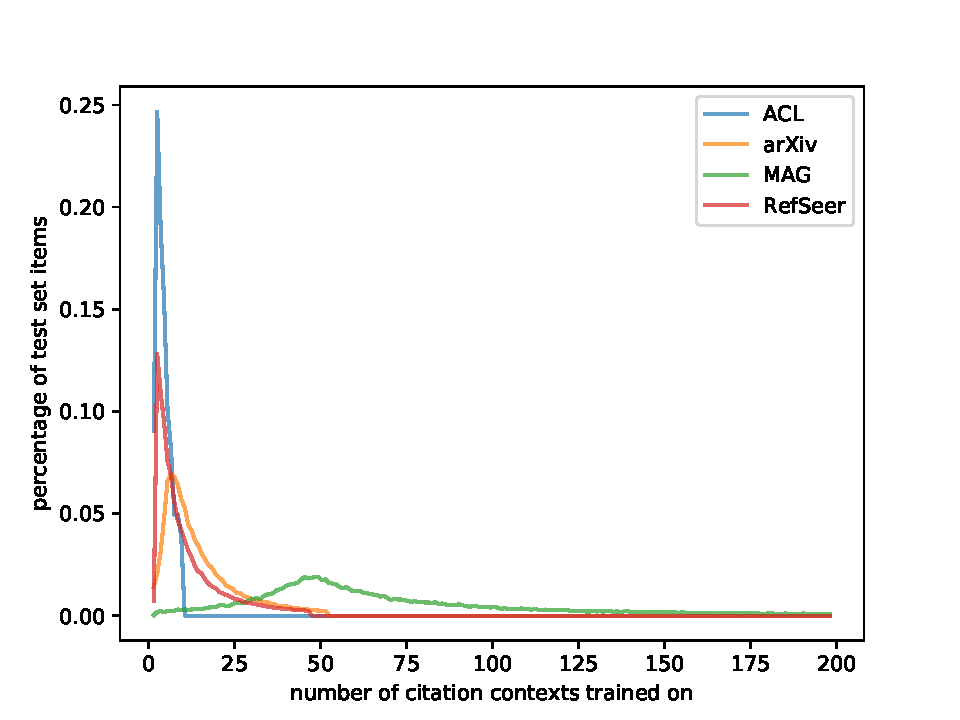
\includegraphics[width=.8\textwidth]{figures/evaluation/comparison_contexts_per_cited_doc.pdf}
  \label{fig:evalcomp}
  \caption{Number of citation contexts per recommendation candidate.}
\end{figure}

\begin{figure}
  \centering
    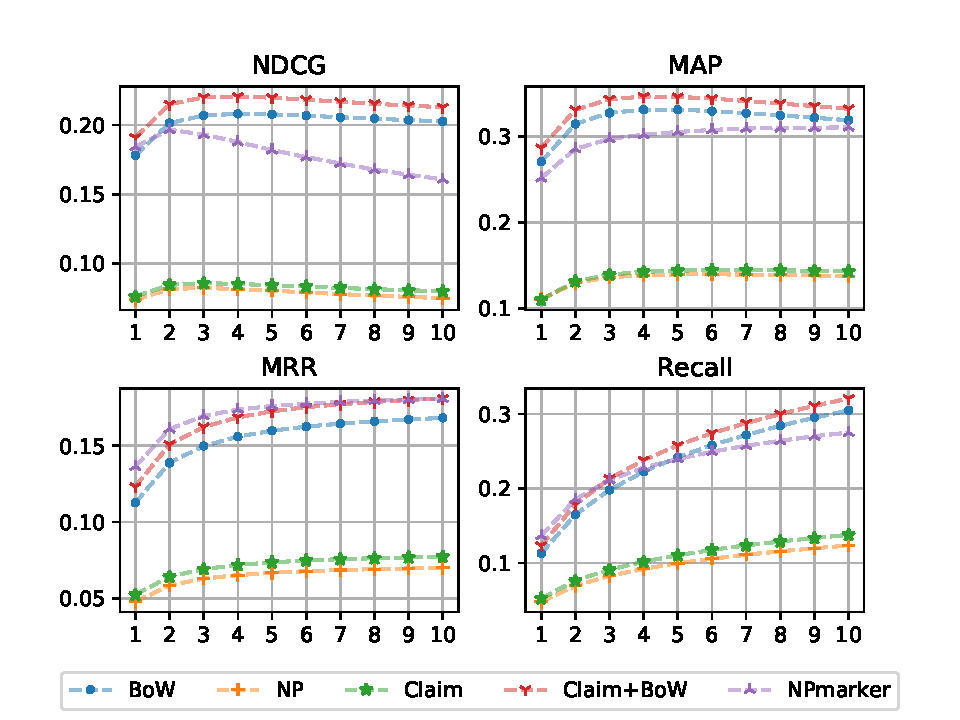
\includegraphics[width=.9\textwidth]{figures/evaluation/arXiv_CS_select.pdf}
  \label{fig:evalarxiv}
  \caption{Evaluation using arXiv.}
%\end{figure}

%\begin{figure}
  \centering
    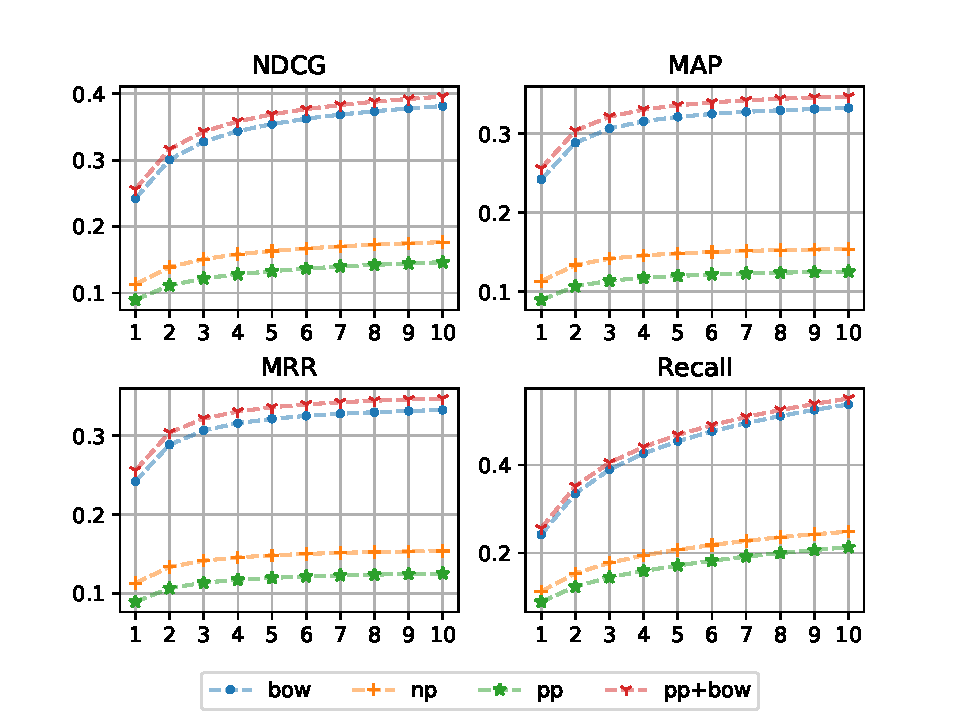
\includegraphics[width=.9\textwidth]{figures/evaluation/MAG_CS_es_wAbs_3M.pdf}
  \label{fig:evalmag}
  \caption{Evaluation using the MAG.}
\end{figure}

\begin{figure}
  \centering
    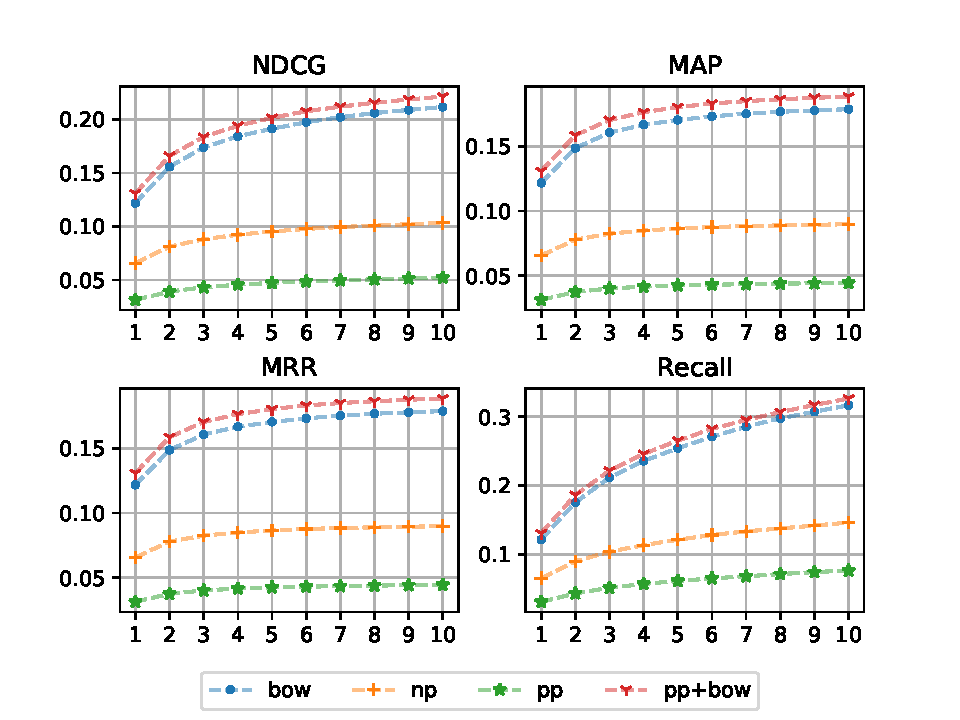
\includegraphics[width=.9\textwidth]{figures/evaluation/RefSeer.pdf}
  \label{fig:evalrefseer}
  \caption{Evaluation using RefSeer.}
%\end{figure}

%\begin{figure}
  \centering
    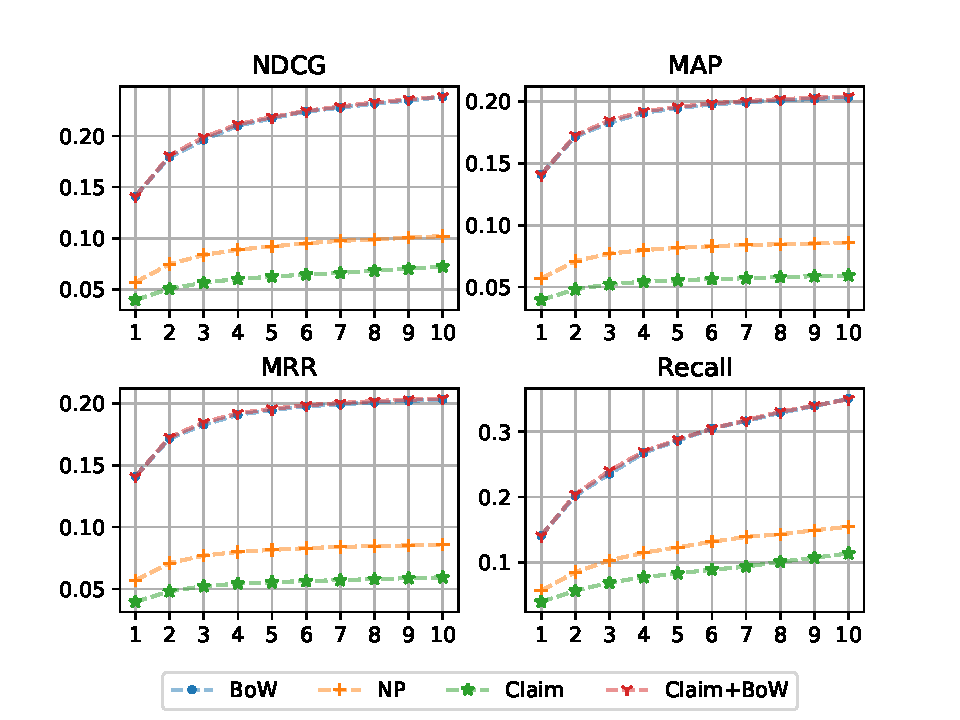
\includegraphics[width=.9\textwidth]{figures/evaluation/ACL.pdf}
  \label{fig:evalacl}
  \caption{Evaluation using ACL-ARC.}
\end{figure}

TFIDF baseline being hard to beat is consitent with observation in \cite{Beel2017}

\section{Online evaluation}\label{sec:oneval}
online online
